
\documentclass[twoside,twocolumn]{article}

\usepackage{blindtext} 
\usepackage{pgf-pie}
\usepackage[sc]{mathpazo}
\usepackage[T1]{fontenc} 
\linespread{1.05} 
\usepackage{microtype} 
\usepackage[english]{babel} 
\usepackage{graphicx}
\usepackage{centernot}
\usepackage{mathtools}
\usepackage{amsfonts}
\usepackage{algorithm}
\usepackage{array}
\usepackage{breqn}
\usepackage[noend]{algpseudocode}
\algrenewcommand\algorithmicrequire{\textbf{Input:}}
\newcommand\ddfrac[2]{\frac{\displaystyle #1}{\displaystyle #2}}
\graphicspath{ {images} }
\usepackage[hmarginratio=1:1,top=32mm,columnsep=20pt]{geometry} 
\usepackage[hang, small,labelfont=bf,up,textfont=it,up]{caption}
\usepackage{booktabs} 
\usepackage{lettrine} 
\usepackage{enumitem} 
\setlist[itemize]{noitemsep}
\usepackage{multicol}
\usepackage{tabularx}
\usepackage{abstract} 
\renewcommand{\abstractnamefont}{\normalfont\bfseries} 
\renewcommand{\abstracttextfont}{\normalfont\small\itshape}

\usepackage{titlesec} 
\renewcommand\thesection{\Roman{section}}  
\renewcommand\thesubsection{\roman{subsection}}
\titleformat{\section}[block]{\large\scshape\centering}{\thesection.}{1em}{} % Change the look of the section titles
\titleformat{\subsection}[block]{\large}{\thesubsection.}{1em}{} 

\usepackage{fancyhdr} 
\pagestyle{fancy} % All pages have headers and footers
\fancyhead{} % Blank out the default header
\fancyfoot{} % Blank out the default footer
\fancyfoot[RO,LE]{\thepage} % Custom footer text

\usepackage{titling} % Customizing the title section

\usepackage{hyperref} % For hyperlinks in the PDF

\setlength{\droptitle}{-4\baselineskip} % Move the title up

\pretitle{\begin{center}\Huge\bfseries} % Article title formatting
	\posttitle{\end{center}} % Article title closing formatting
\title{A data-driven approach for the analysis of SARS-CoV-2 mutations} % Article title
\author{%
	\textsc{Samuele Del Bello, Stefano Destro, Alessio Frezza,}\\
	\textsc{Rita Numeroli, Carlos Santillán} \\[1ex] % Your name
	\textsc{Supervisor: Pietro Pinoli PhD}\\
	\normalsize  Applied Statistics Project - Politecnico di Milano \\
}
\date{July 25th, 2022} 
\renewcommand{\maketitlehookd}{%
	\begin{abstract}
		\noindent We consider the problem of extracting meaningful mutation patterns from a SARS-CoV-2 mutation dataset by exploiting the large quantity of data available. In particular, we focus on identifying synergistic mutation pairs (or groups) via an association rule mining approach. This study also explores the main characteristics of the most significant lineages and their relationships. Finally, we show that the process of clade discovery can be aided or partially automated via hierarchical clustering techniques.
	\end{abstract}
}

\begin{document}
	\maketitle
	
	\section{Introduction}
	
	The wide availability of SARS-CoV-2 tests has provided us with large amounts of data on the virus' amino acid and RNA mutations. We study a dataset from Nextstrain\cite{nextstrainbook}, a project that collects data on viral outbreaks. At first, we aimed to find synergistic mutation pairs and perform clustering to find well-defined groups within the lineages; as we explored the data, the connections between these two objectives became clear and merged into one. This report is organized into four parts:
	\begin{itemize}
		\item Overview and exploration of the dataset 
		\item Explanation of the methods used to analyze the data
		\item Data analysis and pattern recognition
		\item Conclusion and further analysis
	\end{itemize}
	On the advice of our supervisor, we decided to ignore the RNA mutations since the information they conveyed was, in significant part, already embedded into the amino acid mutations.
	%------------------------------------------------
	
	\section{Overview of the dataset}
	
	In its raw form, our dataset contained 4 million samples, with columns relative to the species of the subject, country, date, mutations w.r.t. the original Wuhan sequence (both RNA and amino acid), sequence length, lineage, and clade. We briefly explain some of the terminology.
	\begin{itemize}
		\item \textbf{Clade: }Group of organisms that share a common ancestor. Can be seen as a branch in a phylogenetic tree.
		\item \textbf{Lineage: } A single line of descent or linear chain in the phylogenetic tree.
		\item \textbf{Amino acid mutation: } A change in the proteins of the sample w.r.t. the original Wuhan sequence. If in protein S the 614th amino acid changed from D to G, the mutation would be labeled as S:D614G. Similar rules apply to RNA mutations\cite{nomenclature}.
	\end{itemize}
	In Table 1, we see a fragment of the dataset (excluding some columns). Usually, any given sample can have up to 200 mutations. 
	\begin{table}
		\caption{Fragment of the dataset}
		\centering
		\renewcommand{\arraystretch}{1.2} % enlarge line spacing
		\begin{tabular}{|c|c|c|c|}
			\hline
			Clade & Lineage & Amino acid mutations \\
			\hline
			21E  & P.3& N:R203K, N:G204R, ... \\
			20J & B.1.1.7 & N:D3L, N:R203K, ...\\
			20J & B.1.1.7 & N:D3L, N:P151L, ...\\
			20J & P.1.15 & M:H125Y, N:P80R, ...\\
			21G & C.37 & N:P13L, N:A119P, ...\\
			\hline
		\end{tabular}
	\end{table}
	The dataset also contains 1397 lineages and 25 clades. However, we quickly realized that only 15 lineages had more than 50K samples (a healthy amount to apply the methods explained later). The pie chart in Figure 1 shows the largest lineages w.r.t. the number of samples. 
	\begin{figure}
		\caption{Pie chart of lineages w.r.t. number of samples} \label{piechart}
		\begin{tikzpicture}
			\pie{15/AY.4, 13/B.1.1.7, 8/BA.1, 6/BA.1.1, 5/AY.103, 4/AY.44, 2/AY.3,47/Under 100K}
		\end{tikzpicture}
	\end{figure}
	This already shows that our analysis will mainly focus on those lineages. To get a panoramic view of the data, we can also look at the entire phylogenetic tree in Figure 2. The colors are assigned according to the clade, but it also contains all possible lineages. It is worth noting that some level of data cleaning and processing was necessary. Many samples were irrelevant (e.g., non-human subject) or incomplete (e.g., no lineage). We exploited the missing data column, which indicates how many amino acids were not sequenced in the samples. Through this, we filtered half a million samples with a high level of incompleteness, leaving 3.5 million samples. \\
	The final step was converting the mutation data (string format, comma-separated mutations) to many binary columns, each being a mutation. So we transformed the initial dataset into a binary format by filtering mutations that appeared at least 0.01\% of the time within each lineage. In Table 2, we see the transformed dataset.
	\begin{figure}[h]
		\caption{Phylogenetic tree of SARS-CoV-2}
		\label{tree}
		\centering
		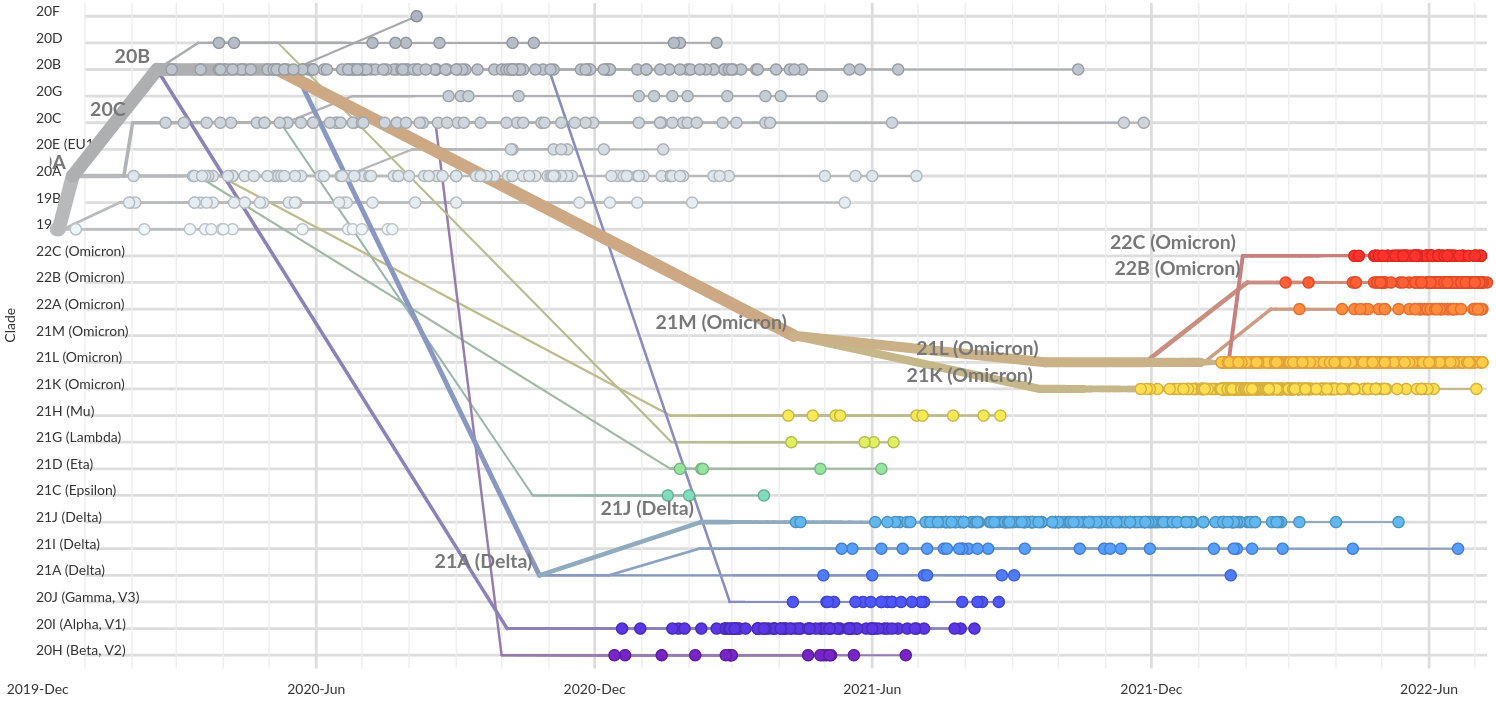
\includegraphics[width=70mm, height=40mm]{covidtree.png}
	\end{figure}
	\begin{table}
		\caption{Transformed dataset}
		\centering
		\renewcommand{\arraystretch}{1.2} % enlarge line spacing
		\begin{tabular}{| c | c | c | c | }
			\hline
			Lineage & N:D3L & N:R203K & N:G204R\\
			\hline
			P.3& 0 & 1 & 1 \\
			B.1.1.7 & 1 & 0&0 \\
			B.1.1.7 & 1 & 0&0 \\
			P.1.15 & 0 & 0 &0\\
			C.37 & 0 & 0 &0\\
			\hline
		\end{tabular}
	\end{table}
	\\The last part of the exploration looked at each lineage's mutation frequencies. Figure 3 shows a barplot of the mutation percentages within AY.103 (196K samples).
	\begin{figure}[h]
		\caption{Mutation percentages in AY.103}
		\label{ay103barplot}
		\centering
		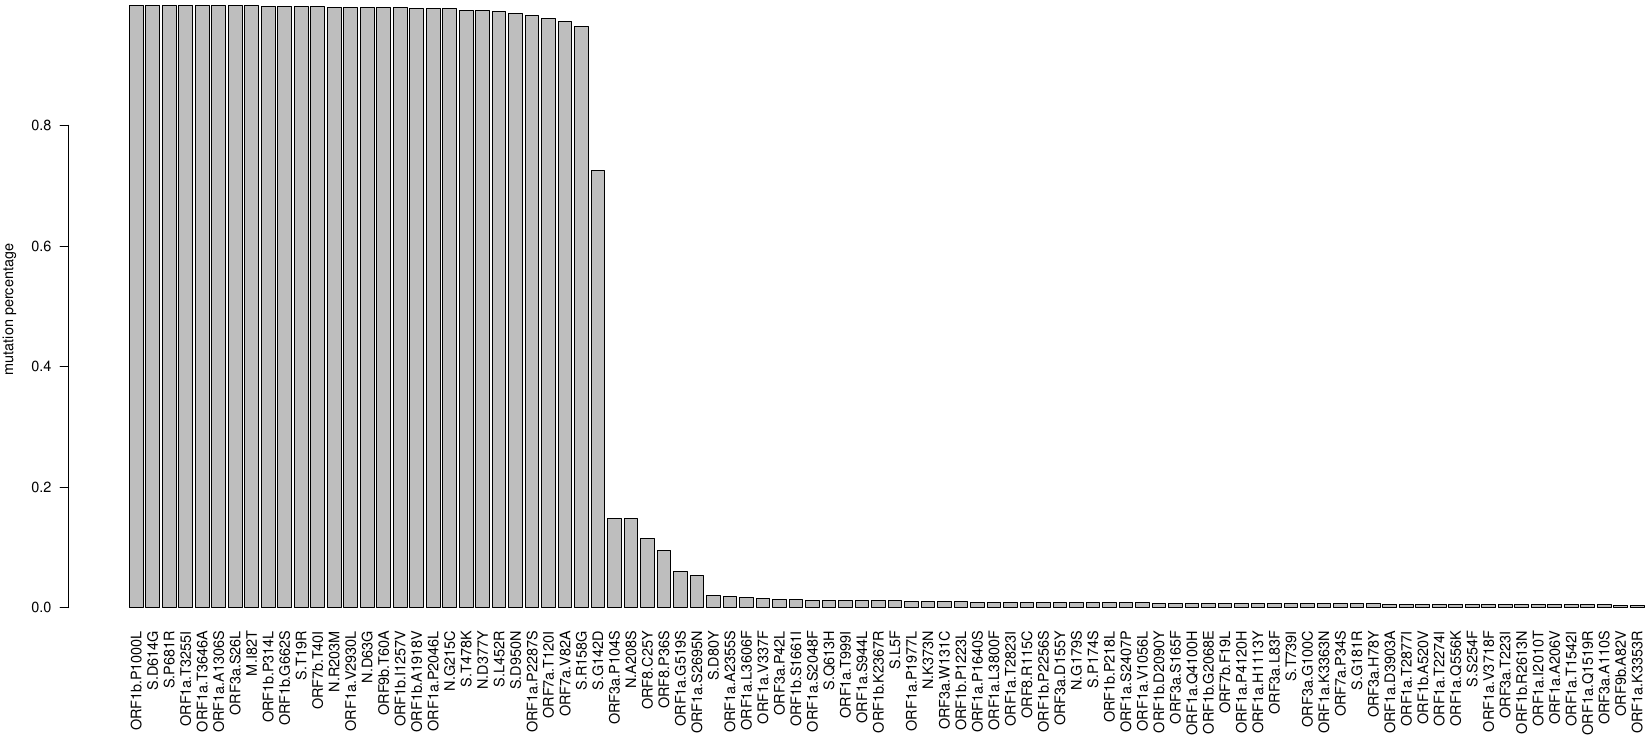
\includegraphics[width=70mm, height=40mm]{ay103barplot.png}
	\end{figure}
	As we can see, some mutations are predominant, and very few are present between 10\% and 90\%. The rest are almost insignificant, but as we will see later, they might help explain subgroups within the lineage. The mutation frequency distribution is similar in other lineages; again, some mutations are almost always present, and the rest have a presence below 1\%. At this stage, we can already see that the most present mutations within each lineage are the ones that characterize it.
	%------------------------------------------------
	
	\section{Methods and techniques}
	
	The first problem we tackled was identifying recurring pairs of mutations. So we could see it as a classification task with Support Vector Machines or Logistic Regression (interpreting the weights). However, we saw that approaches such as Association Rule Mining\cite{armpaper} and TF-IDF\footnote{Term frequency–inverse document frequency.}\cite{tfidf} adapted better to the binary nature of the data.
	We briefly explain methods not treated during the course, specifically ARM\footnote{Association rule mining.}. The three methods we used are
	\begin{itemize}
		\item Association rule mining with the Apriori algorithm
		\item Principal component analysis
		\item Hierarchical clustering with Ward linkage\cite{ward}
	\end{itemize}
	\subsection{Association Rule Mining}
	Consider each sample as a \textquotedblleft transaction\textquotedblright$\,$that contains certain items (i.e., mutations). We provide some definitions:
	\begin{itemize}
		\item \textbf{Association rule:} An expression $X$ $\rightarrow$ $Y$, where $X$ and $Y$ are disjoint mutation subsets. 
		\item \textbf{Support:} The support of a subset of mutations \textit{X}, denoted by 
		\begin{align*}
			sup(X)
		\end{align*} is the number of transactions (or samples) in a transaction dataset \textbf{D} that contain \textit{X}. In Table 3 the subset \{A\} has support 2 since it appears in two transactions. Subset \{B, C\} has support 1. It is an estimate of the joint probability of the items in \textit{X}. The support of rule $\{B\} \rightarrow \{C\}$ is 1.
		\item \textbf{Confidence:} The confidence of a rule is an estimate of the conditional probability that a transaction contains $Y$ given that it contains $X$.
		\begin{align*}
			conf(X \rightarrow Y) = P(X|Y) = \frac{P(X \land Y)}{P(X)}
		\end{align*}
		It can also be seen as $\frac{sup(X \cup Y)}{sup(X)}$. In Table 3 the confidence of $\{B\} \rightarrow \{C\}$ is 0.5. Confidence can be a misleading metric in some cases, it is mostly used for filtering very unlikely rules, but not for assessing their quality.
		\item \textbf{Lift:} Ratio of the observed joint probability of $X$ and $Y$ to the expected joint probability if they were statistically independent.	
		\begin{align*}
			lift(X \rightarrow Y) = \frac{P(X\cup Y)}{P(X)\cdot P(Y)} = \frac{conf(X\rightarrow Y)}{rsup(Y)}
		\end{align*}
		Where $rsup(Y) = \frac{sup(X\cup Y)}{|\mathbf{D}|}$. If it is equal to 1, then the rule is expected since the support of single mutations is enough to deduce it. We are interested in rules with lift much above or below 1, which would mean the rule is unexpected from the support. It can also be seen as a linear correlation index. 
		\item \textbf{Order: } The number of elements in the rule. For example, a rule with order 3 might be $\{A,B\} \rightarrow \{C\}$, it includes both antecedent and consequent. The number of rules of order $n + 1$ will always be much larger than those of order $n$.
	\end{itemize}
	\begin{table}
		\caption{Example binary dataset}
		\centering
		\renewcommand{\arraystretch}{1.2} % enlarge line spacing
		\begin{tabular}{| c | c | c | c | }
			\hline
			Transaction & Mut. A & Mut. B & Mut. C\\
			\hline
			1& 0 & 1 & 1 \\
			2 & 1 & 0&0 \\
			3 & 1 & 0&0 \\
			4 & 0 & 1 &0\\
			5 & 1 & 0 &1\\
			\hline
		\end{tabular}
	\end{table}
	Figure 4 shows the support v. confidence plot of rules extracted from a 40K balanced dataset of the four largest lineages. The hue indicates the lift value. Figure 5 shows the two-key plot\footnote{Same as support v. confidence plot, but the color is assigned according to the order.}. As noted before, the number of rules of order 3 is overwhelmingly larger than those of orders 1 and 2.
	\begin{figure}[h]
		\caption{Support v. confidence plot for 82K rules}
		\label{ruleslift}
		\centering
		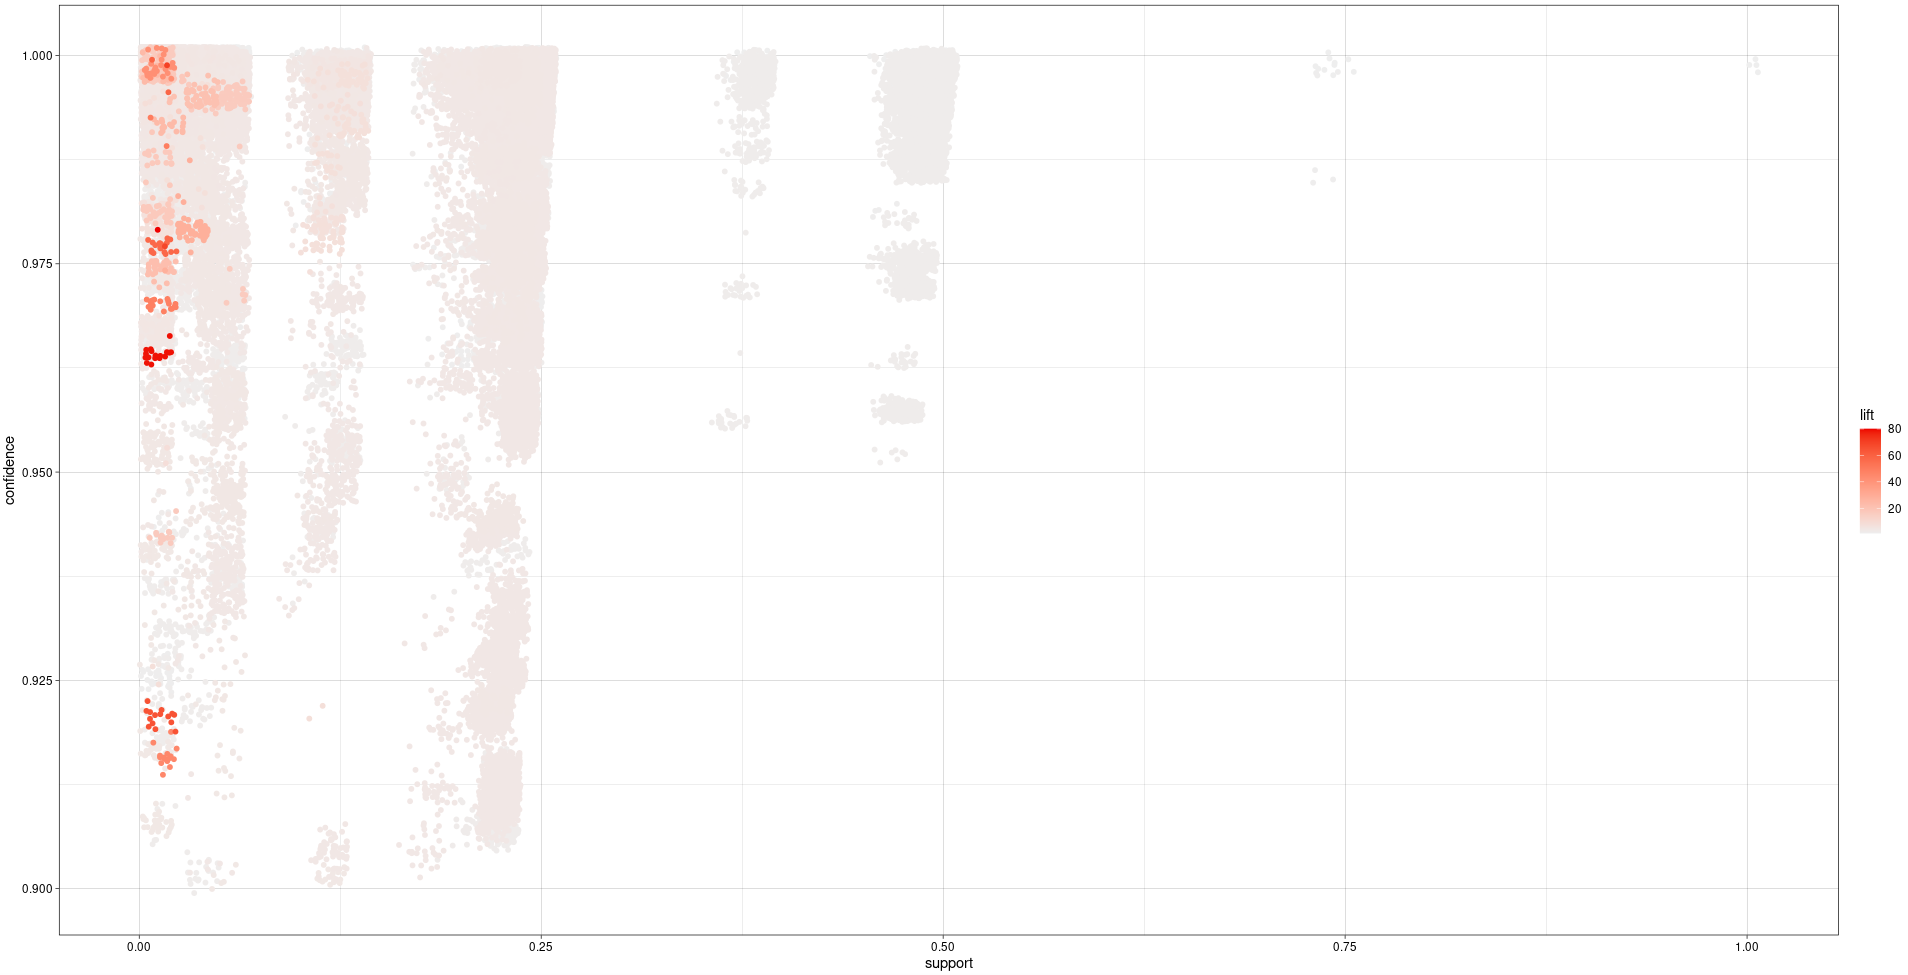
\includegraphics[width=70mm, height=40mm]{rules1.png}
	\end{figure}
	\begin{figure}[h]
		\caption{Two-key plot}
		\label{rulesorder}
		\centering
		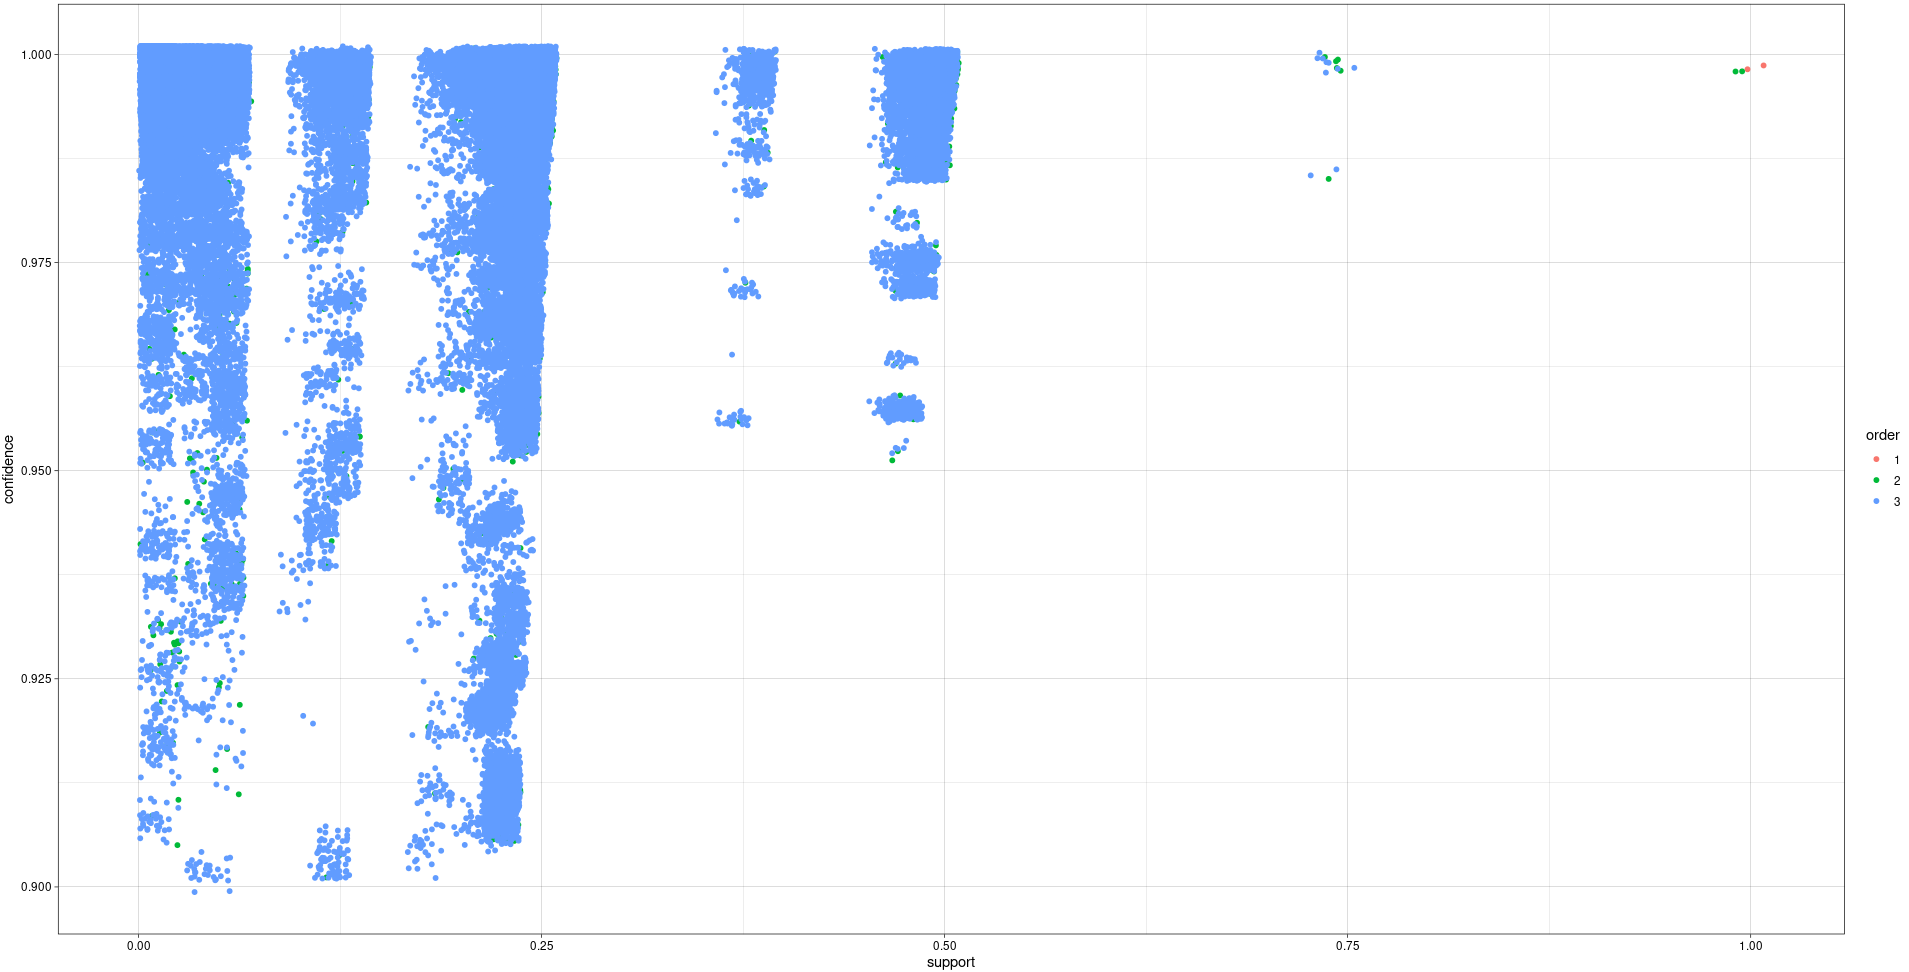
\includegraphics[width=70mm, height=40mm]{rules2.png}
	\end{figure}
	\\
	ARM can help us identify non-obvious patterns within the lineages. However, given the number of all possible rules (larger even than the power set of mutations), we need to resort to an efficient algorithm for rule mining.
	\subsection{Apriori algorithm}
	We only briefly explain the intuition behind Apriori. For a complete introduction, see the original paper\cite{apriori}. We want to extract rules whose antecedent $X$ has a minimum support of $minsup$. We can exploit this requirement to reduce the rule search space drastically. The Apriori property states:
	\begin{quote}
		\textit{All non-empty subsets of a frequent mutation set $X$ must also be frequent.} 
	\end{quote}
	$X$ is frequent if $sup(X) > minsup$. The following observation is also fundamental; if a mutation $A$ is added to a non-frequent mutation set $X$, the resulting set cannot occur more frequently than $X$. Therefore $X\cup \{A\}$ is non-frequent as well, since $P(X\cup\{A\}) < \frac{minsup}{|\mathbf{D}|}$. These properties are used to prune branches off the rule tree that we know, a priori, are non-frequent. 
	\\
	Although the standard Apriori R implementation is relatively fast, other algorithms offer comparable or superior performance depending on certain assumptions, such as FP-Growth\cite{fpgrowth} and LCM\cite{lcm}. 
	\subsection{Hierarchical clustering and PCA}
	The large number of features led us to perform dimensionality reduction for visualization; this was performed via PCA. Unfortunately, in most lineages at least 5 PCs were needed to explain 50\% or even less of the variability, and up to 15 or 20 to explain 80\%. \\
	We resorted to hierarchical clustering despite the large number of data (e.g., computing the distance matrix over 100K+ samples is infeasible with 8 GBs of RAM). This decision was taken because of the positive results obtained with Ward linkage, subsequently confirmed by our qualitative assessment of the pairs plot on the PCs. Finally, we tackled the previous issue by using random sampling.
	\section{Data analysis and Pattern Recognition}
	This section is divided into two parts:
	\begin{itemize}
		\item Identification of patterns within single lineages and association rules
		\item Clade discovery
	\end{itemize}
	\subsection{Identification of patterns within single lineages and association rules}
	
	We aimed to apply association rules directly to large segments of the dataset. However, this proved unfruitful since the generated rules were too many to filter, even by lift. So we decided to study subsets of individual lineages instead. It is important to note that we performed a repeated sampling of 10K transactions and the following results are consistent throughout all samplings, except for negligible differences. \\We wanted to visualize the data, so we performed PCA and looked at the pairs plot. Figure 6 shows the scree plot after applying PCA on 10K randomly selected samples from AY.103.
	\begin{figure}[h]
		\caption{Scree plot for 10K samples from AY.103}
		\label{screeplot1}
		\centering
		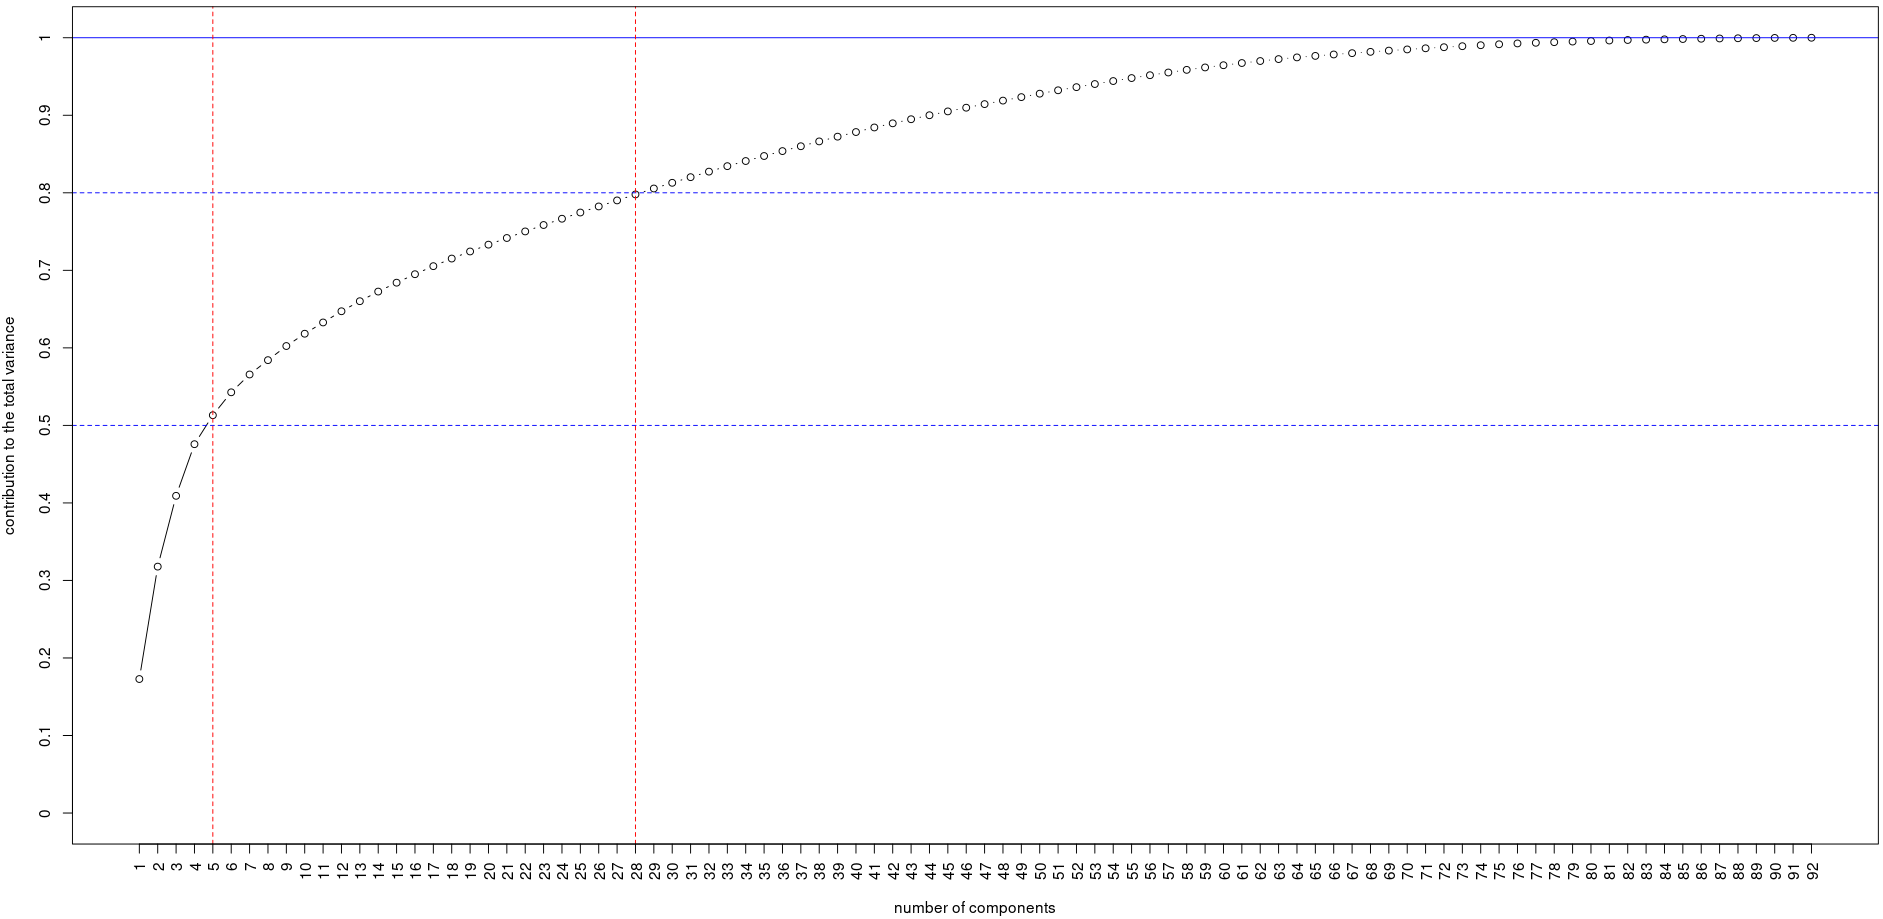
\includegraphics[width=70mm, height=40mm]{scree.png}
	\end{figure}
	We see that the first 5 PCs explain only 50\% of the variability, while we need 28 PCs to explain 80\%. Also, since the features are a form of categorical data, it is rather challenging to provide a thorough interpretation of the loadings. Figure 7 shows the pairs plot of the first 4 PCs (approx. 48\%).
	\begin{figure}[h]
		\caption{Pairs plot of first 4 PCs}
		\label{pairs}
		\centering
		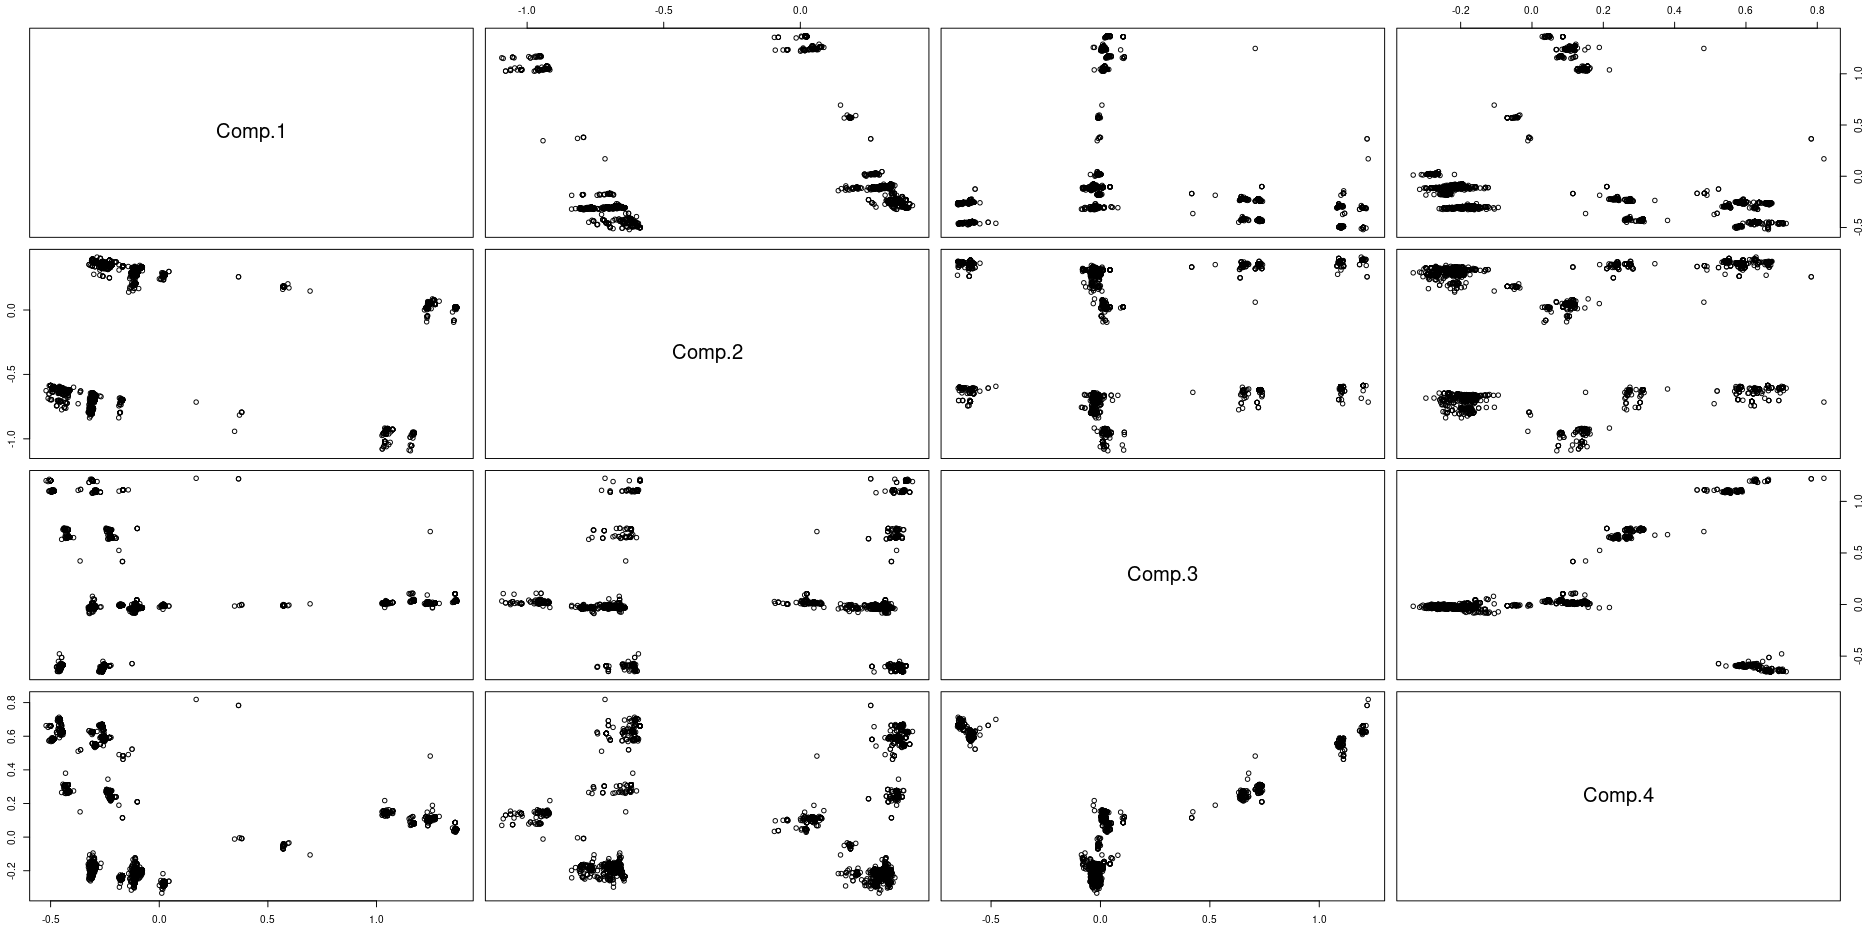
\includegraphics[width=70mm, height=40mm]{pca1.png}
	\end{figure}
	We can see that there might be some clusters. To better observe the density of the data (many points are superimposed since many samples are identical except for a few mutations), we add a gaussian noise with a standard deviation of 0.025. Figure 8 shows the pairs plot with jitter.
	\begin{figure}[h]
		\caption{Pairs plot with jitter}
		\label{pairsjitter}
		\centering
		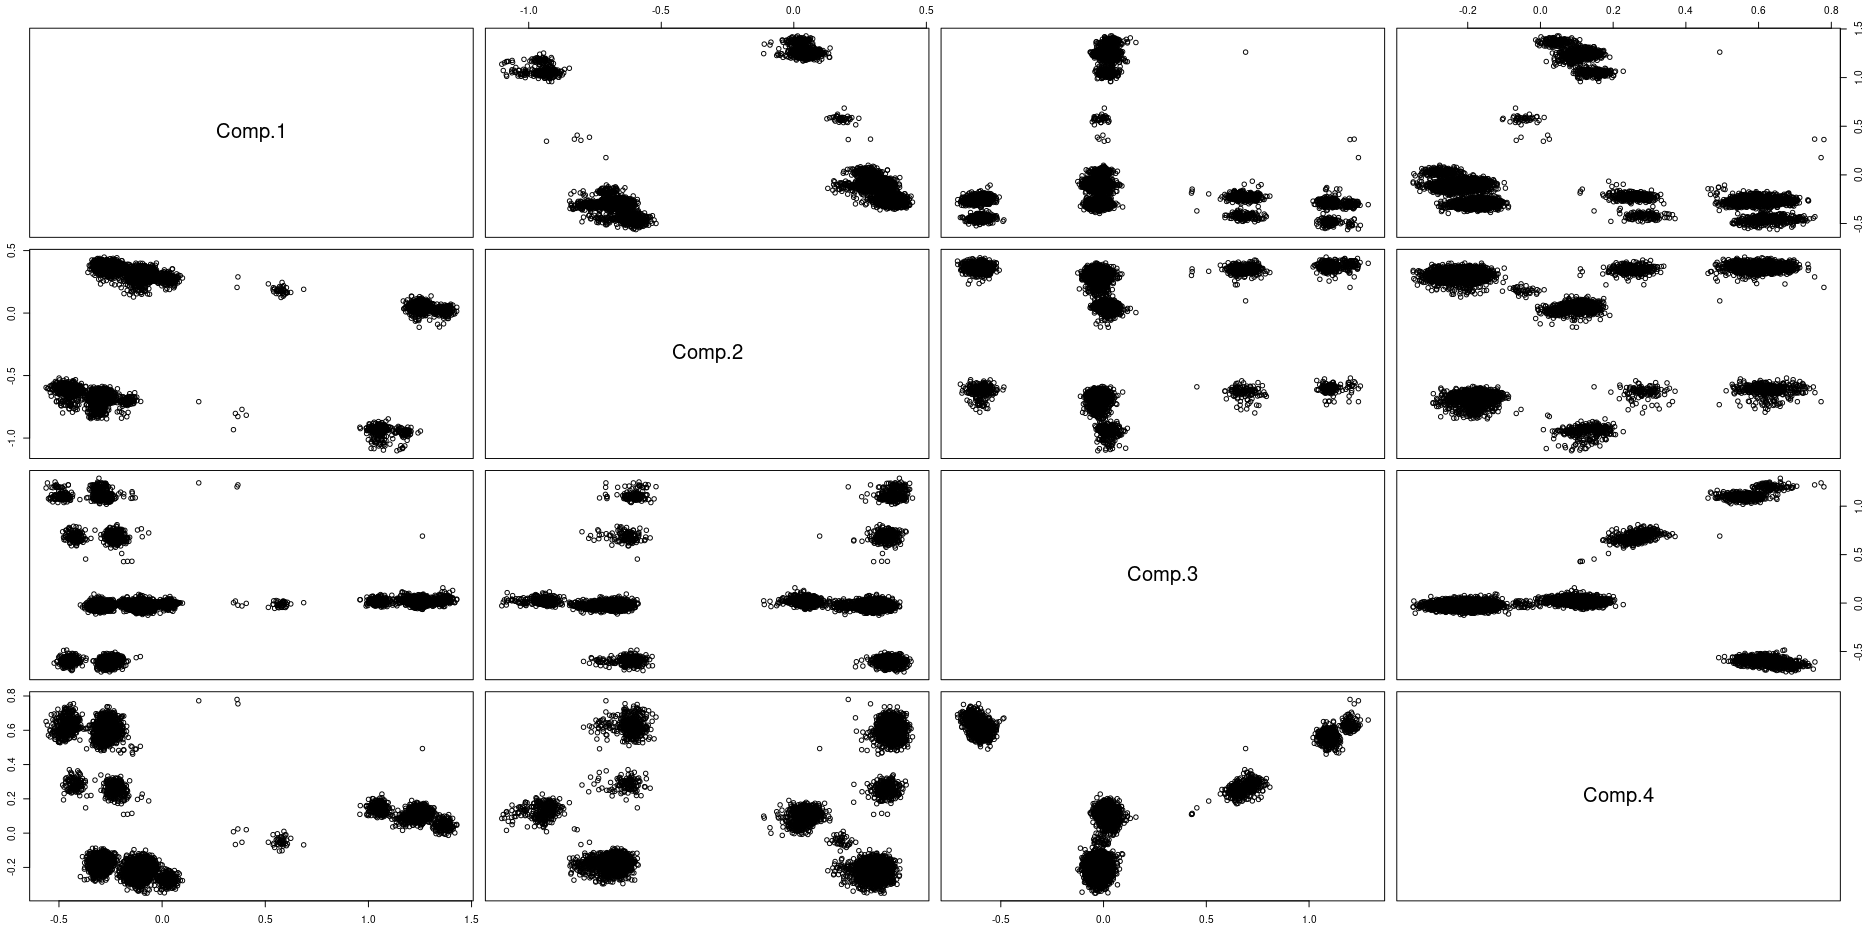
\includegraphics[width=70mm, height=40mm]{pairsjitter.png}
	\end{figure}\\
	We proceed with hierarchical clustering on the original features using Ward linkage\footnote{Ward linkage gave much more balanced clusters w.r.t. other types of linkage}. Figure 9 shows the resulting dendrogram.
	\begin{figure}[h]
		\caption{Dendrogram (clustering with Ward linkage)}
		\label{dendrogram}
		\centering
		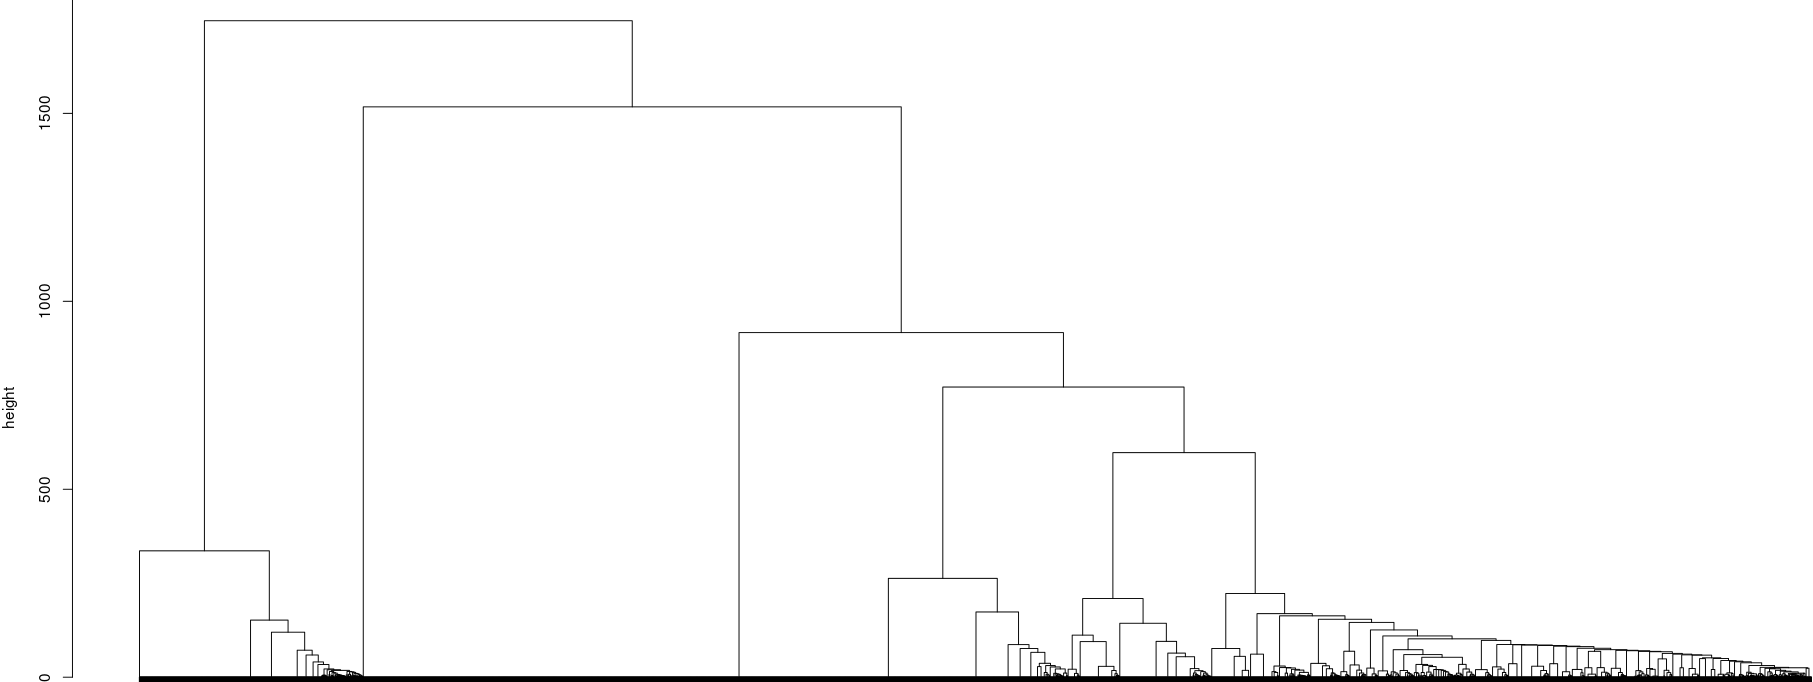
\includegraphics[width=70mm, height=40mm]{dendrogram.png}
	\end{figure}
	In this case, we choose 5 clusters since the dendrogram suggests it is a reasonable number (sizes 2247, 4447, 893, 1338, and 1075). Figure 10 shows the pairs plot, now colored by cluster. 
	\begin{figure}[h]
		\caption{Pairs plot colored by cluster}
		\label{pairscolored}
		\centering
		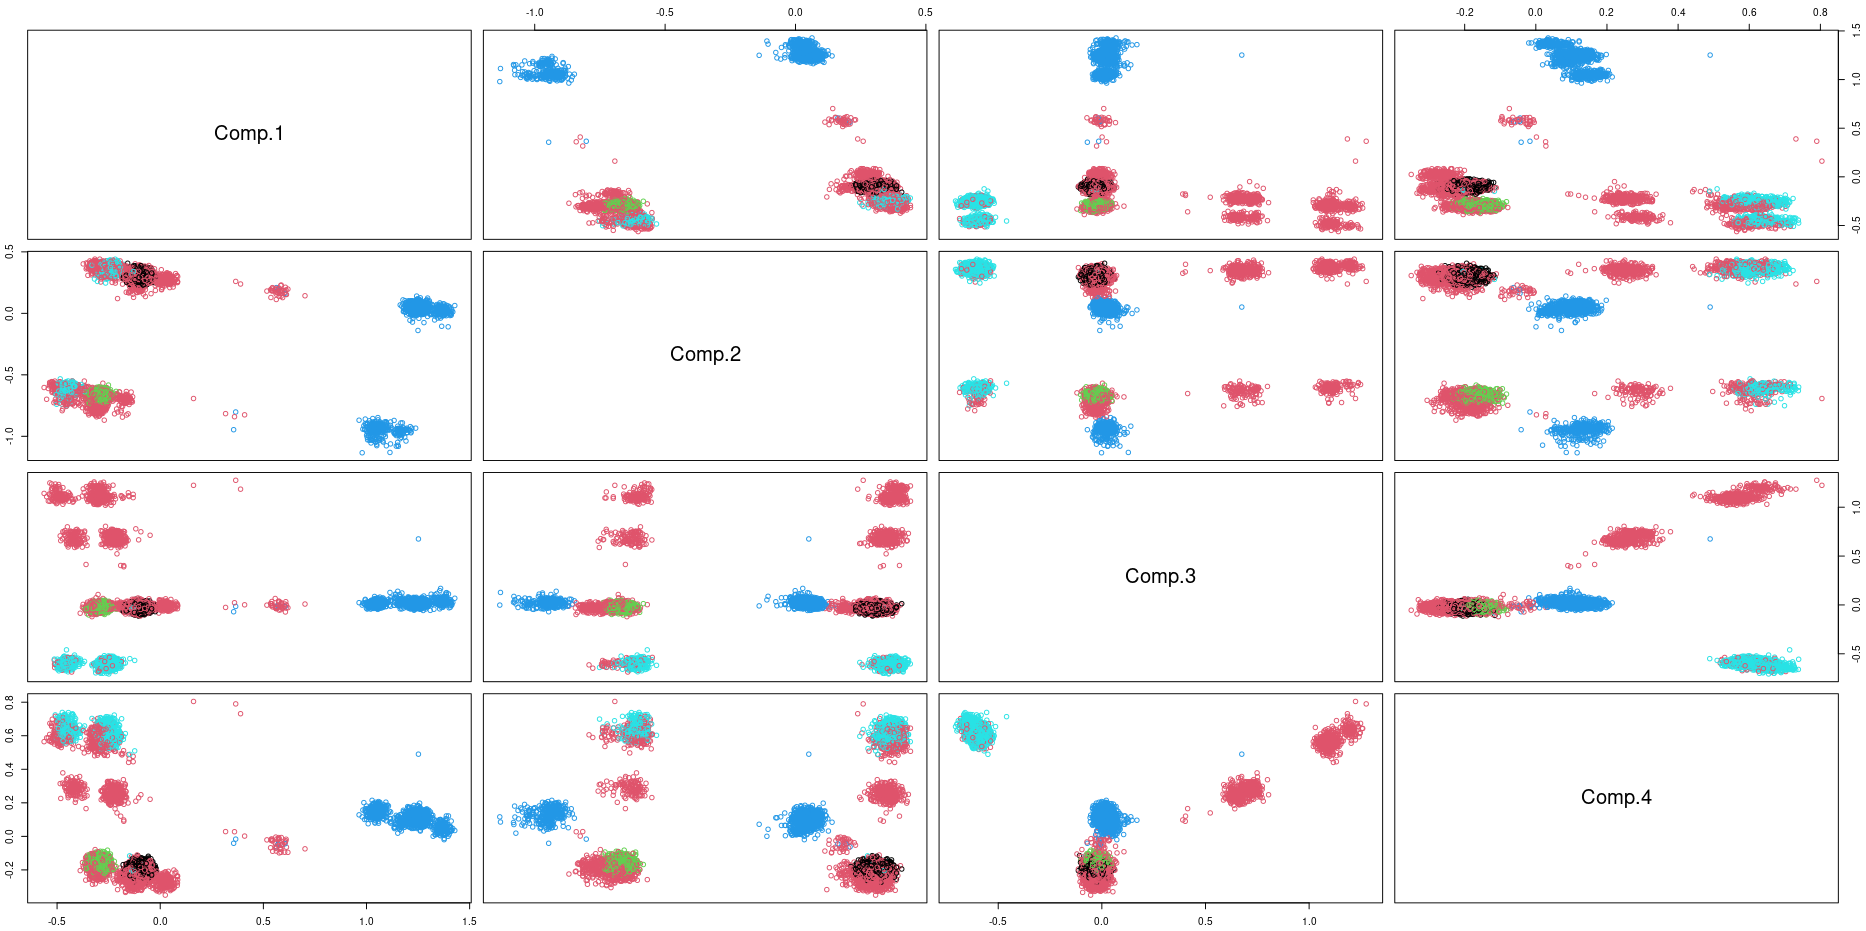
\includegraphics[width=70mm, height=40mm]{pairs2.png}
	\end{figure}\\
	Since the data is high-dimensional, we will not find a perfect match with what we see by eye. However, the procedure found relatively good quality clusters. Therefore, we look at the mutation frequency barplot to visualize each cluster's characteristics. Finally, we see that some clusters are characterized by spikes of specific mutations and by the lack of mutations that are predominant overall. However, these barplots do not state anything about the joint recurrence of these uncommon mutations. For example, in cluster 1, we see a spike of \textit{ORF1a:S2695N} and \textit{ORF8:P36S}. Can we extrapolate a rule of type \{\textit{ORF81a:S2695N}\}$\rightarrow$\{\textit{ORF8:P36S}\}? We run Apriori on 100K samples of AY.103, with $minsup$ 0.01\%, and filter rules whose consequent is \textit{ORF8:P36S}. Table 4 shows rules ending in \textit{ORF8:P36S}. Among the rules ending in \textit{ORF8:P36S}, the one with the highest lift is \{\textit{ORF81a:S2695N}\}$\rightarrow$\{\textit{ORF8:P36S}\} (support of 0.5\%\footnote{Not shown in table for spacing purposes.}), confirming our initial hypothesis. Other rules with similar lift values might be noise or include the one above (Apriori property applies) and require further analysis. 
	
	So we have exploited the information obtained via clustering and redirected our attention to potentially meaningful rules. The biological interpretation is that the mutations may be synergistic or beneficial to the virus or, more importantly, predominant in lineages generated or related to AY.103.
	
	The same procedure can be applied to any given spike and, more generally, to any lineage large enough to allow such a level of random sampling. We have confirmed so, clustering with Ward linkage yields similar results in the main lineages (AY.4, B.1.1.7, BA.1, BA.1.1, AY.44, and AY.3) then confirmed by the pairs plot followed by an interpretation via association rules. 
	\begin{figure}[h]
		\caption{Comparison of frequency barplots. Top to bottom: original barplot, barplot for cluster 1, barplot for cluster 2. Same order of mutations}
		\label{comparison}
		\centering
		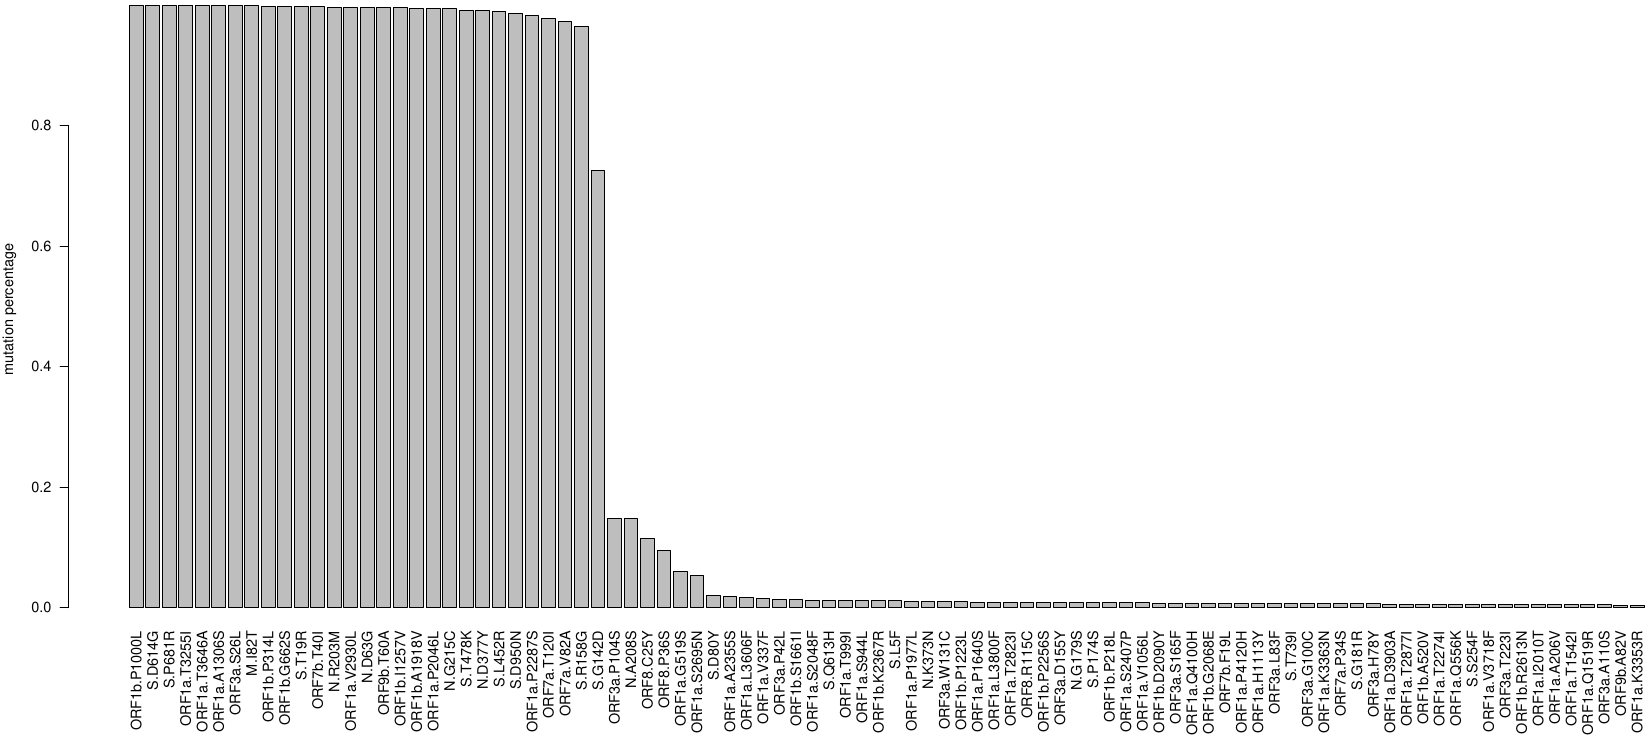
\includegraphics[width=70mm, height=40mm]{c0.png}
		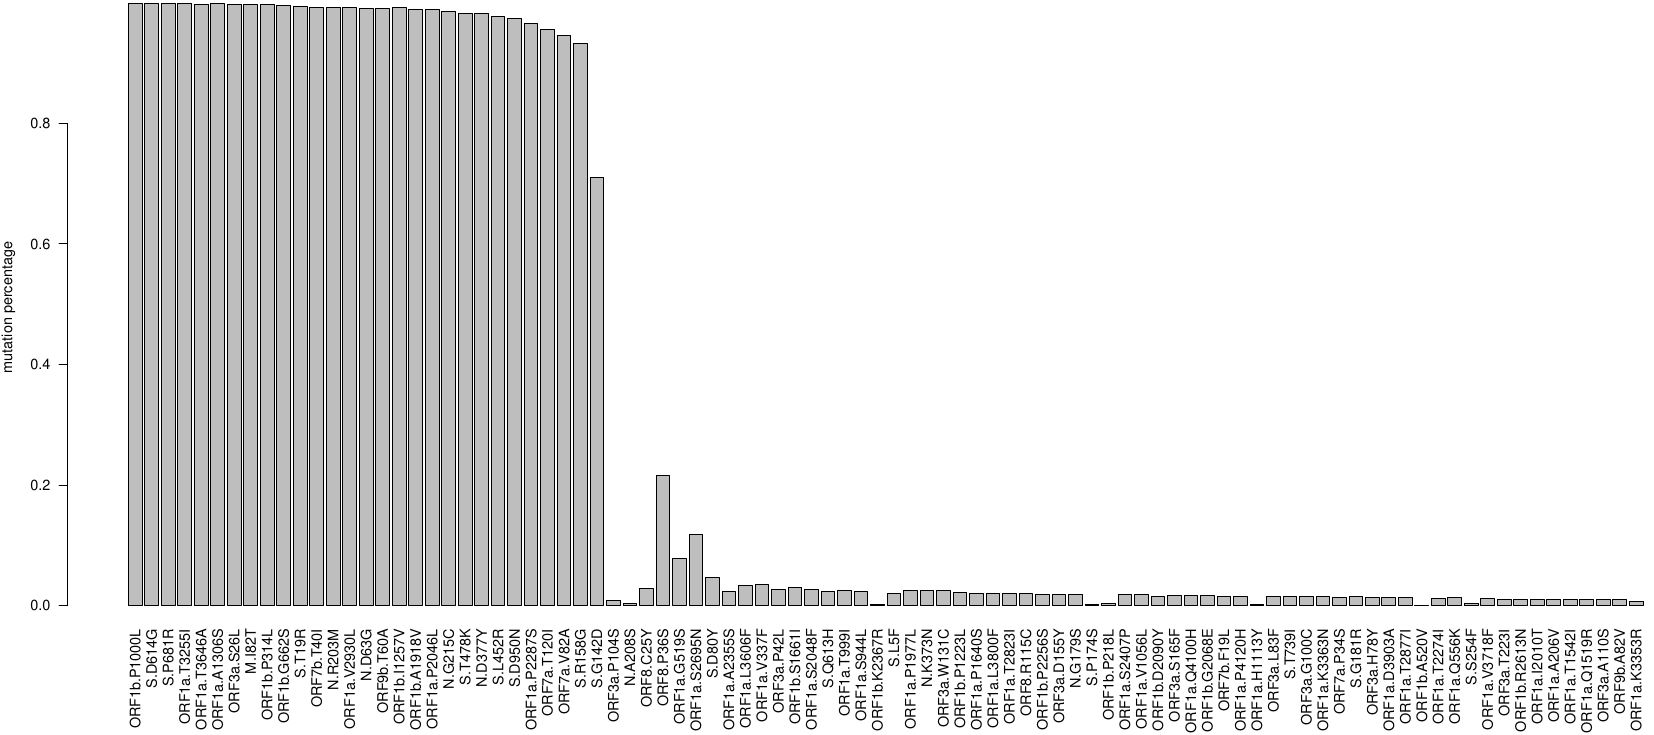
\includegraphics[width=70mm, height=40mm]{c1.png}
		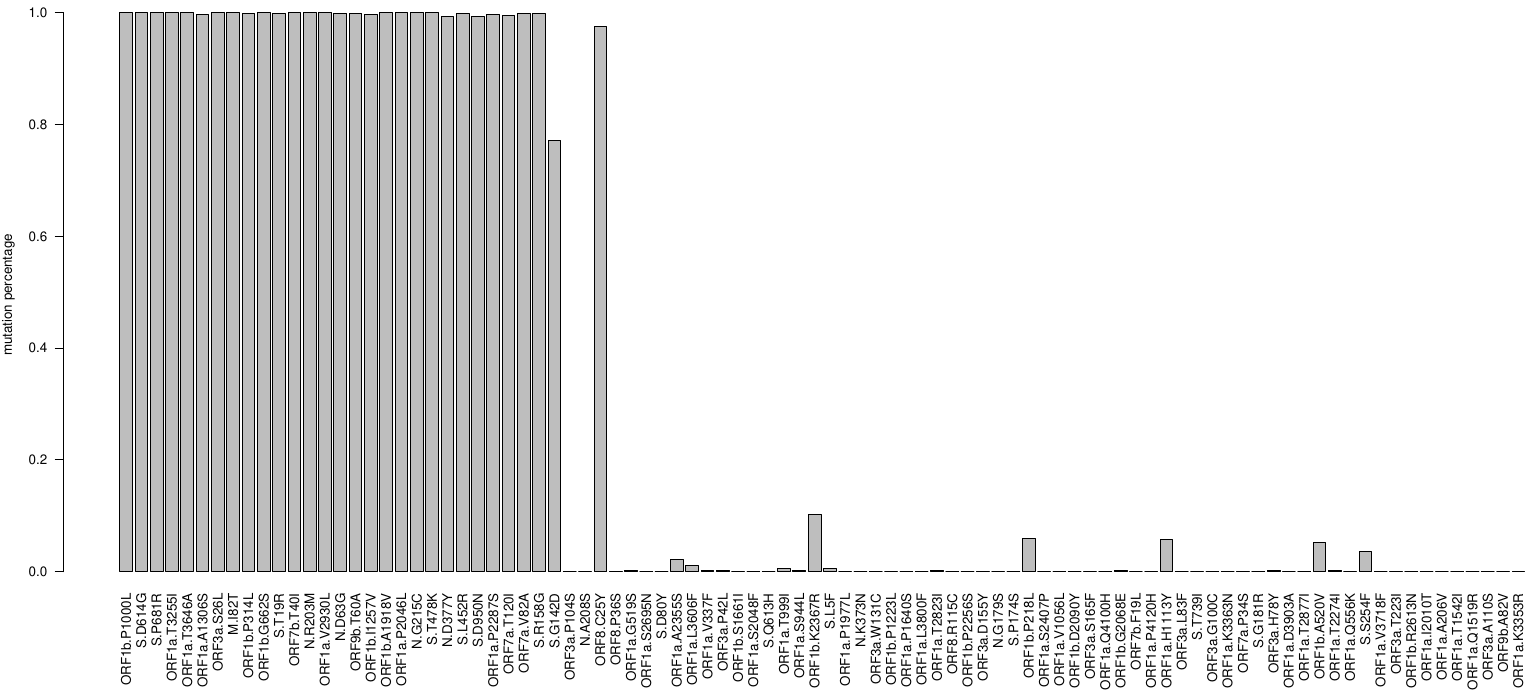
\includegraphics[width=70mm, height=40mm]{c2.png}
	\end{figure}
	\begin{table*}[htb]
		\caption{Rules from AY.103 ending in ORF8:P36S with minsup 0.1\%}
		\label{table:1}
		\renewcommand{\tabcolsep}{2pc} % enlarge column spacing
		\renewcommand{\arraystretch}{1.5} % enlarge line spacing
		\begin{tabularx}{\linewidth}{| c | c | X | X |}
			\hline
			Antecedent & Consequent & Lift & Conf. \\
			\hline
			\{\textit{ORF1a:S2695N}\} & \{\textit{ORF8:P36S}\}  & 10.335 & 0.989\\
			\{\textit{ORF1a:S2695N, ORF1b:P314L}\} & \{\textit{ORF8:P36S}\} & 10.335 & 0.989\\
			\{\textit{ORF1b:P1223L, S:G142D}\} & \{\textit{ORF8:P36S}\} & 9.341 & 0.894\\
			\{\textit{ORF1b:P1223L, S:P681R}\} & \{\textit{ORF8:P36S}\} & 9.294 & 0.889\\
			\{\textit{ORF1b:P1223L, S:D950N}\} & \{\textit{ORF8:P36S}\} & 9.268 & 0.887\\
			\hline
		\end{tabularx}\\[4pt]
	\end{table*}
	\subsection{Clade discovery}
	Another critical problem is lineage assignment and discovery. The current method for SARS-CoV-2 is PANGOLIN\footnote{Phylogenetic Assignment of Named Global Outbreak Lineages.}\cite{pango}. The assignment problem is solved by applying machine learning models, in particular \textquotedblleft pangoLEARN\textquotedblright\cite{pangolearn}. However, the discovery of lineages still needs to be manually curated, and although it leads to more accurate results, it does not fully exploit the large amount of data available. Moreover, no other historical event has provided this amount of data on a specific virus. Can we exploit this as we did for association rules? Unfortunately, this approach is not fine-grained enough to yield accurate results; this is confirmed by our less than satisfactory results for lineage discovery. Can we apply it to clades rather than lineages? We proceed as we did in the previous section.
	\\Figure 12 shows the current clade tree (reduced). We consider five lineages (belonging to three clades) and randomly extract 1600 samples from each (total of 8000 samples). Table 5 shows the lineages and their corresponding clades. We perform PCA and see that the first four principal components explain over 92\% of the variability; this better result w.r.t. to considering a single lineage is due to the intrinsic differences between the lineages. Figure 13 shows the pairs plot colored by lineage and clade.
	\begin{figure}[h]
		\caption{Clade tree (reduced) as of July 2022}
		\label{clades}
		\centering
		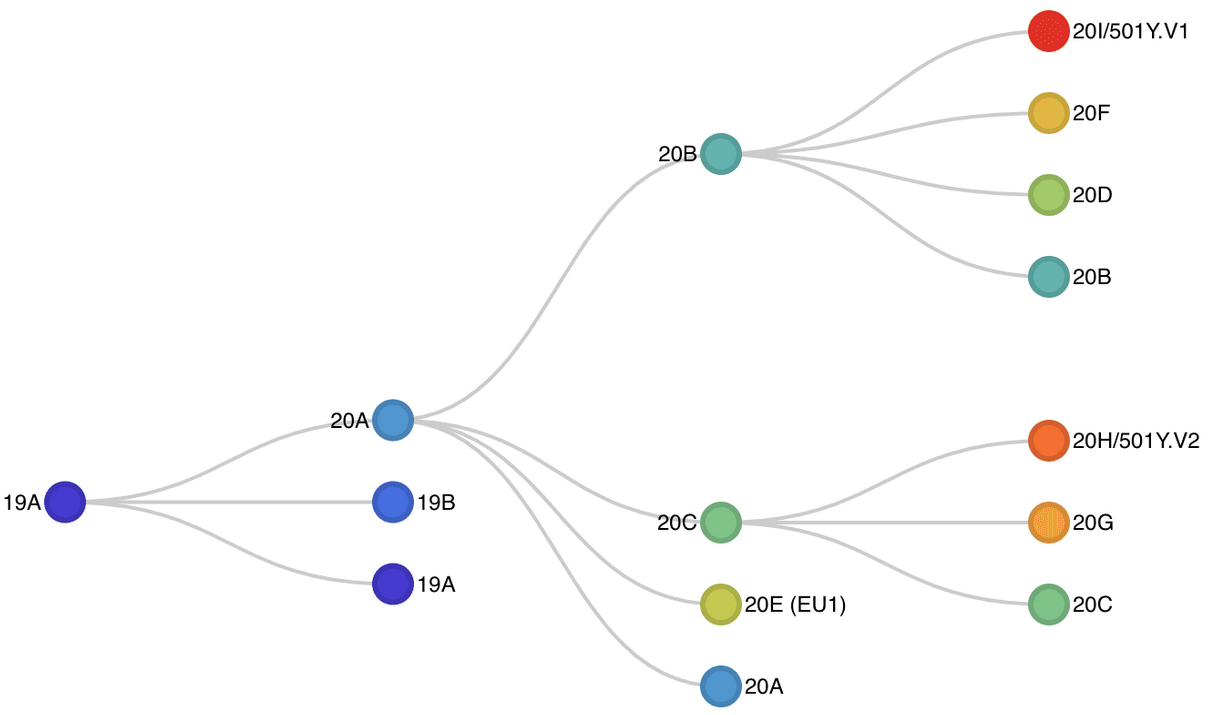
\includegraphics[width=70mm, height=40mm]{clades.png}
	\end{figure}
	\begin{table}
		\caption{Lineage - clade table}
		\centering
		\renewcommand{\tabcolsep}{2pc} % enlarge column spacing
		\renewcommand{\arraystretch}{1.2} % enlarge line spacing
		\begin{tabular}{| c | c |}
			\hline
			Lineage & Clade \\
			\hline
			AY.103 & 21J (Delta) \\
			AY.4 & 21J (Delta) \\
			B.1.1.7 & 20I (Alpha) \\
			BA.1 & 21K (Omicron) \\
			BA.1.1 & 21K (Omicron)\\
			\hline
		\end{tabular}
	\end{table}
	\begin{figure}[h]
		\caption{Pairs plot of prinicipal components. Top to bottom: colored by lineage, colored by clade}
		\label{pairsx}
		\centering
		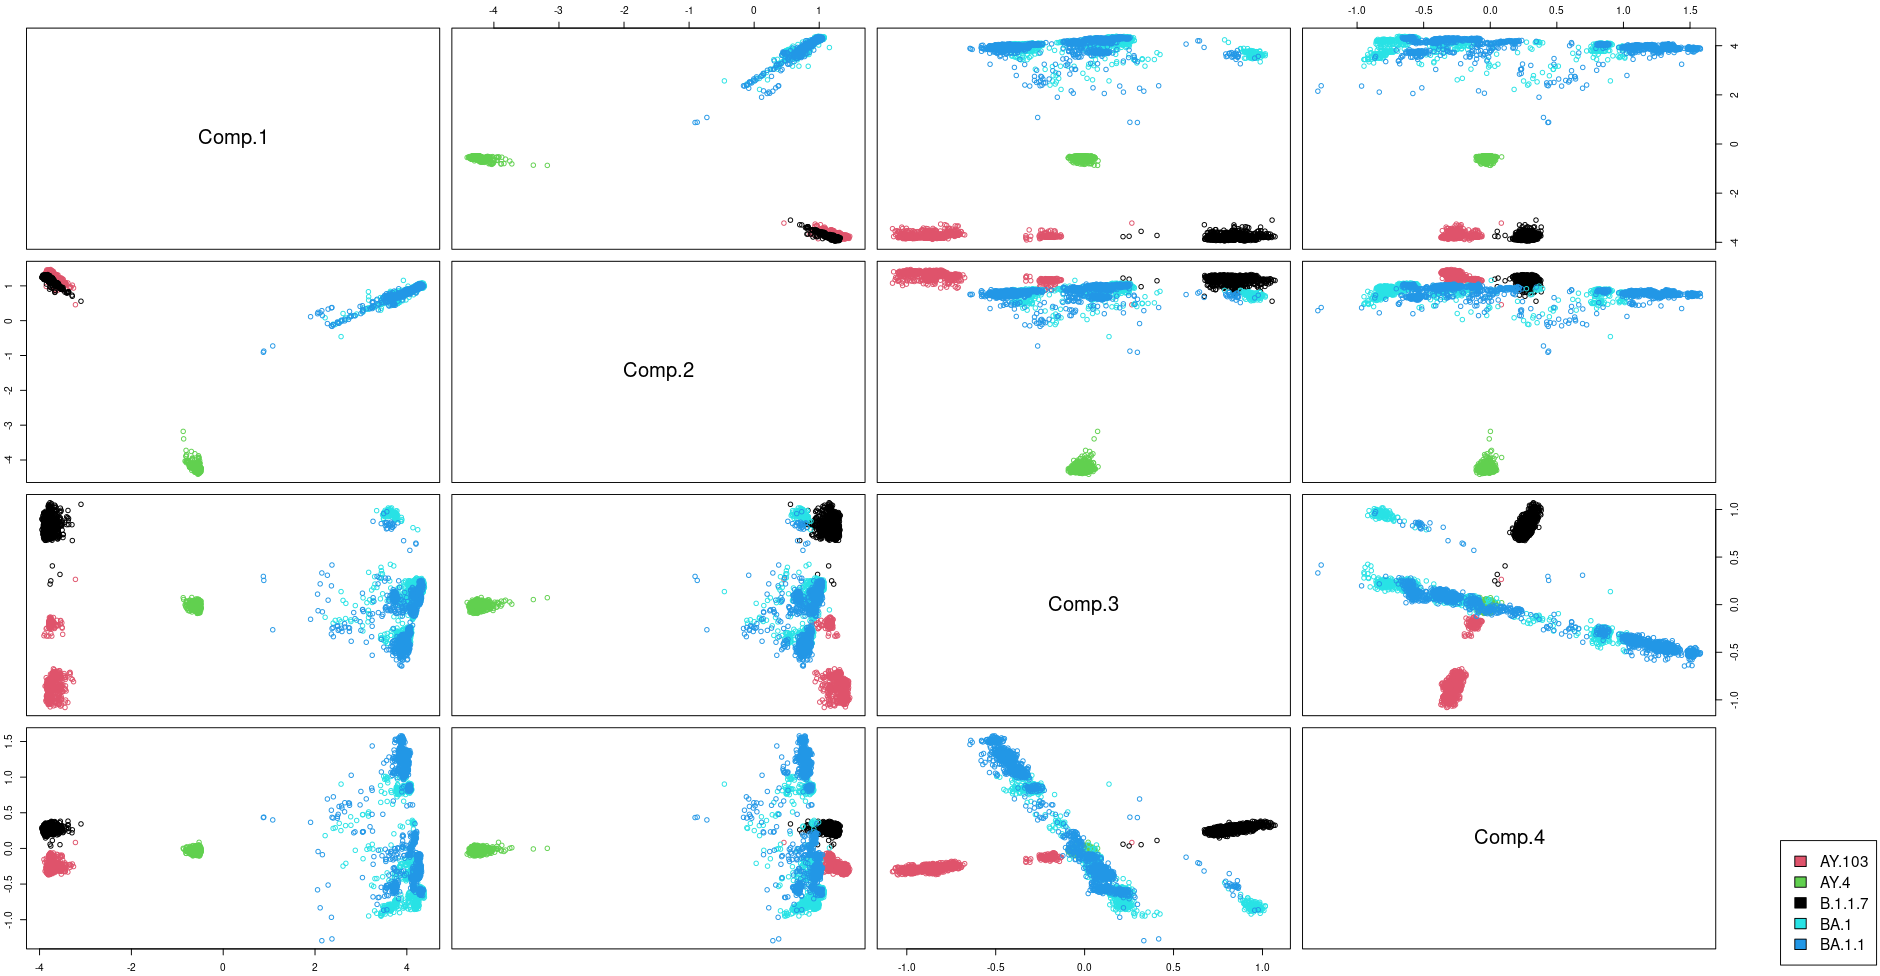
\includegraphics[width=70mm, height=40mm]{pairsx.png}
		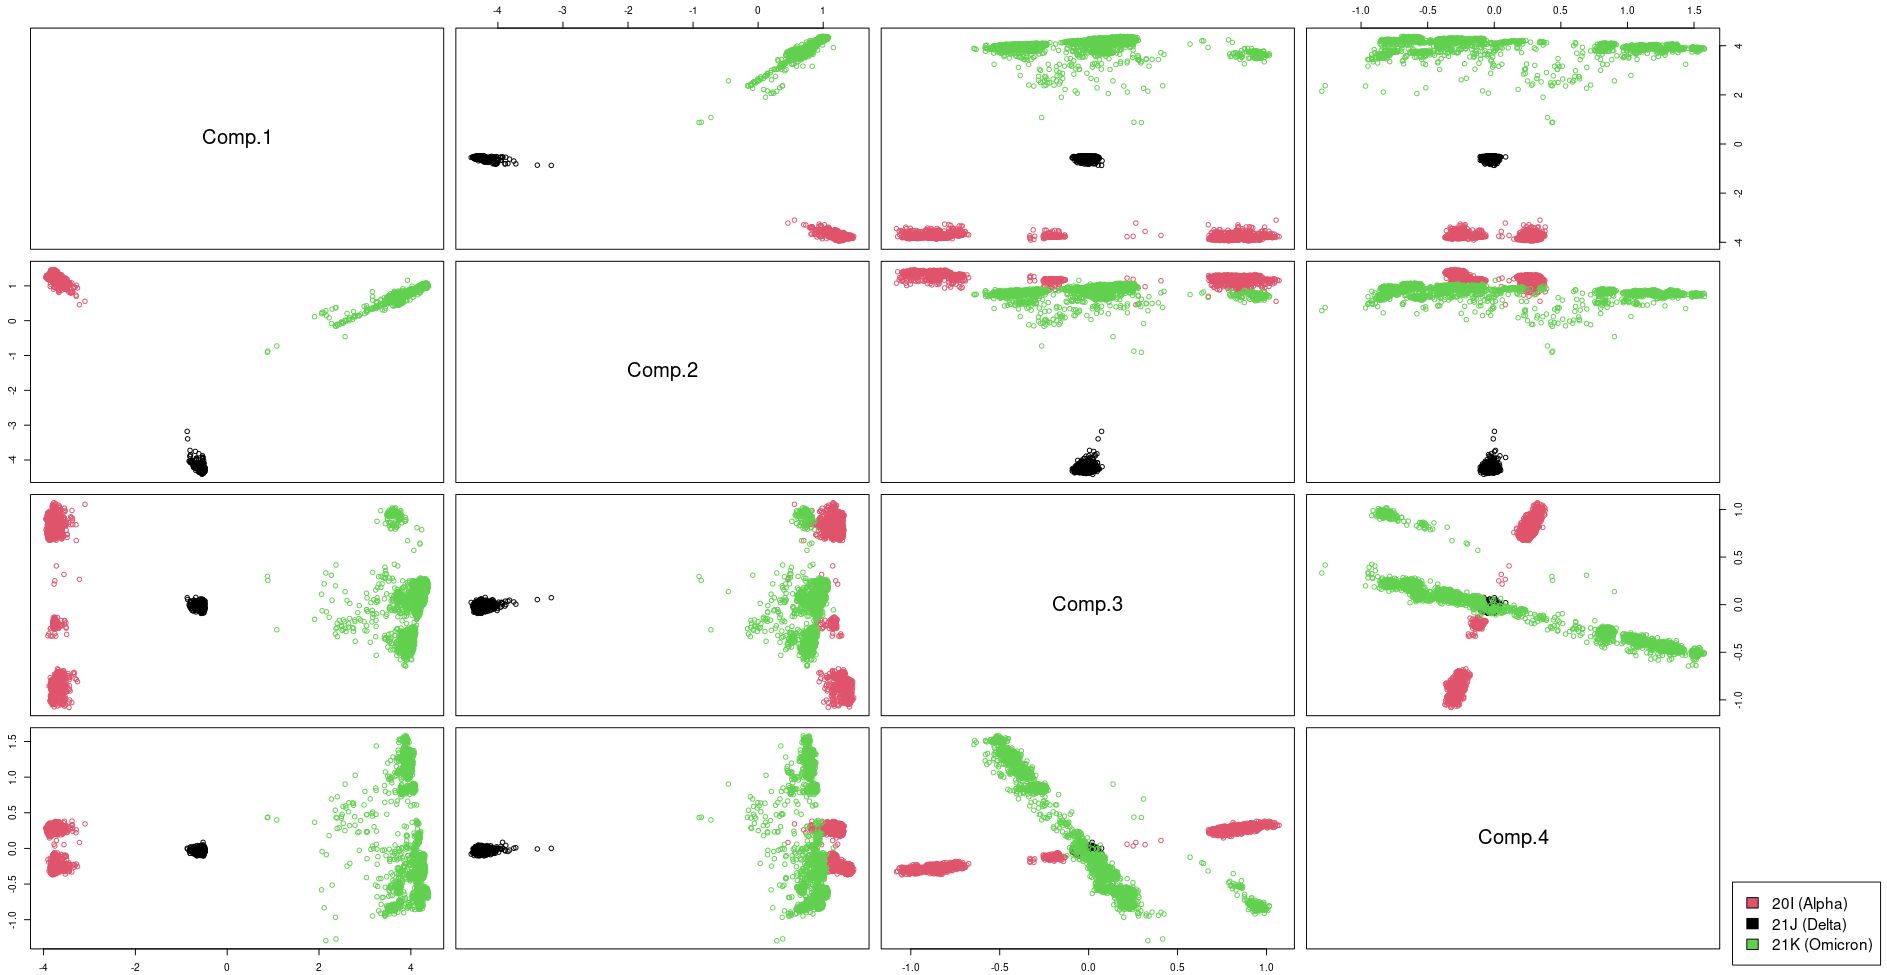
\includegraphics[width=70mm, height=40mm]{pairsx2.png}
	\end{figure}
	The idea is to perform clustering and obtain clusters that follow the clades. Clades are more coarse-grained by nature (there are 25 clades as opposed to over 1000 lineages). Clustering with Ward linkage produces the dendrogram in Figure 14.
	\begin{figure}[h]
		\caption{Dendrogram (clustering on mixed lineage dataset)}
		\label{ward2}
		\centering
		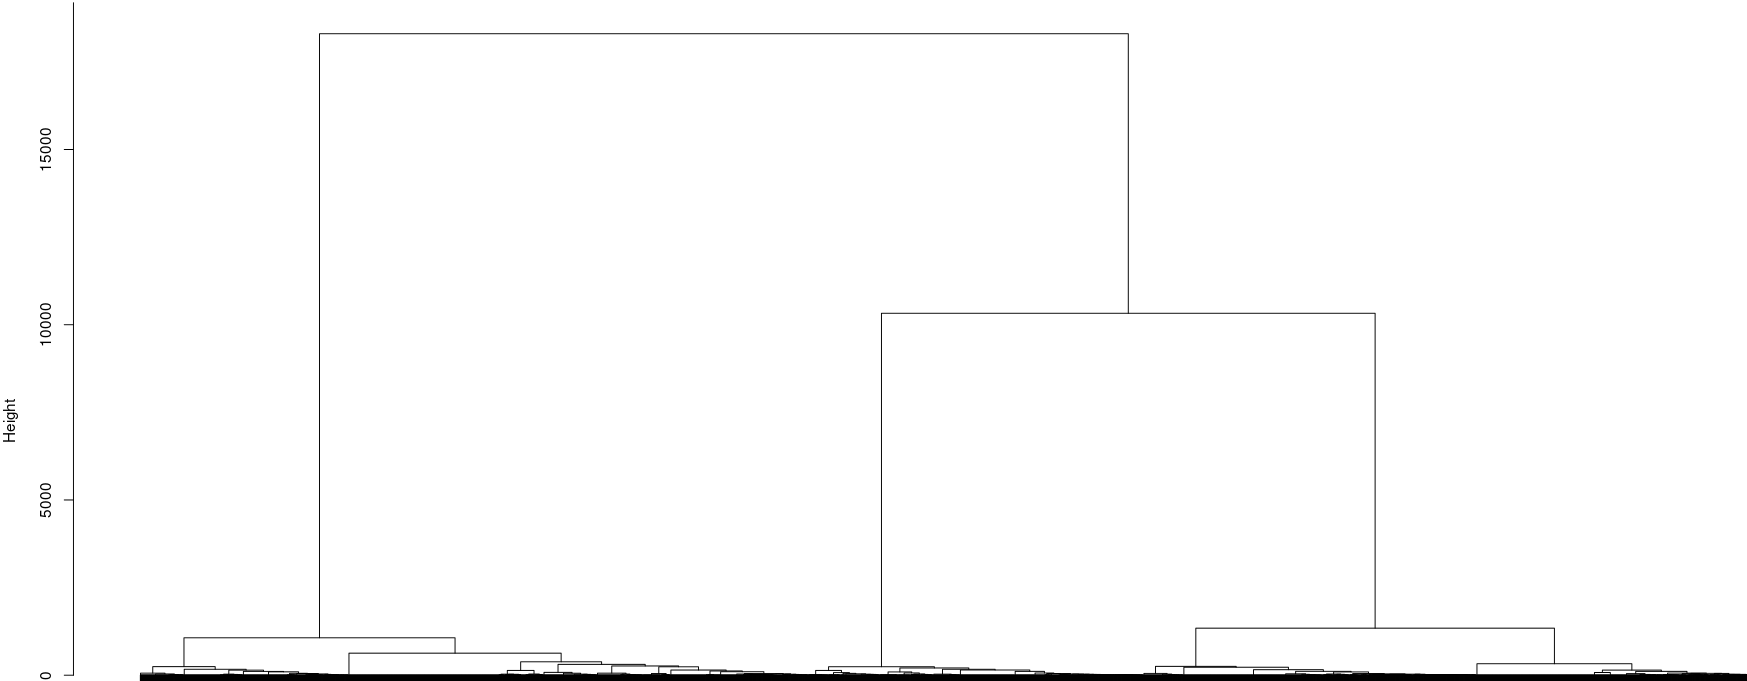
\includegraphics[width=70mm, height=40mm]{ward.png}
	\end{figure}
	The dendrogram suggests the choice of three clusters, the same number of clades we have. Figure 15 shows the pairs plot colored by cluster.
	\begin{figure}[h]
		\caption{Pairs plot colored by cluster}
		\label{pairs3}
		\centering
		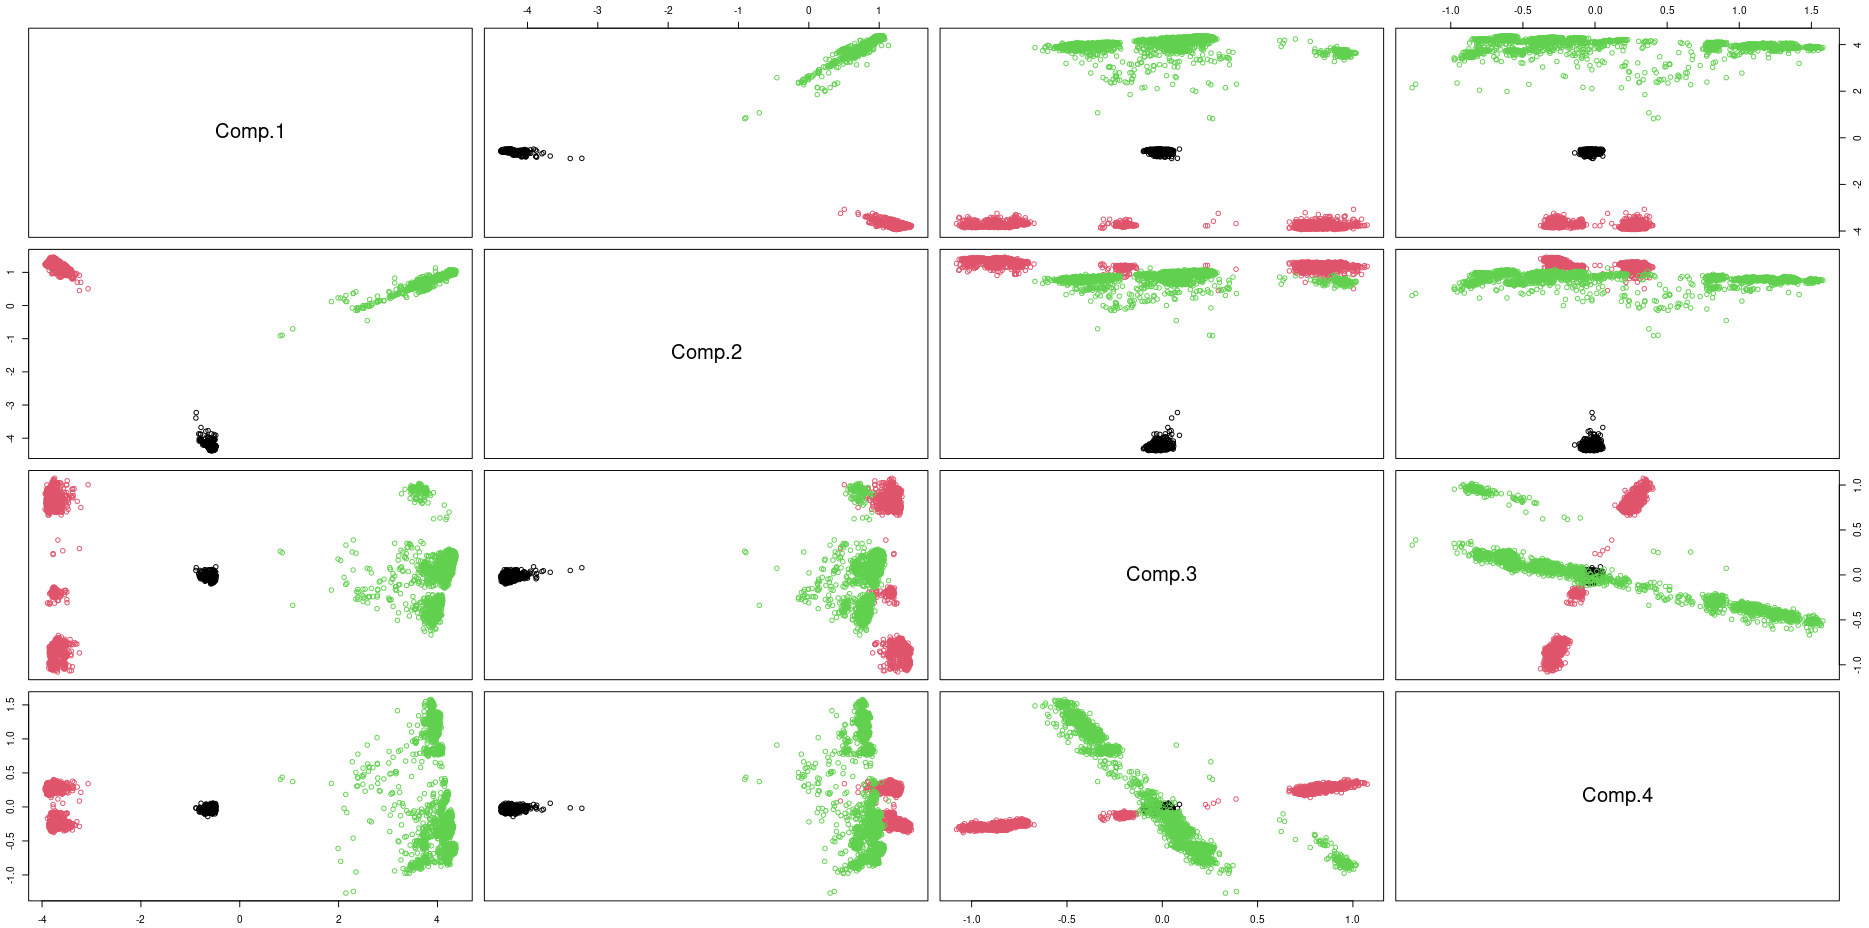
\includegraphics[width=70mm, height=40mm]{pairs3.png}
	\end{figure}
	We observe an almost perfect correspondence with the clade grouping. This result suggests adopting a data-driven approach to aid clade discovery rather than manually curated. It is reasonable to assume that with more sophisticated techniques, we could also apply this pipeline to lineages. 
	It is worth noting that the current clade assignment method is not PANGOLIN but one developed by Nextstrain\cite{cladeassignment}, which closely follows the WHO variant designations (still manually curated). 
	\section{Conclusion and future work}
	We have shown that standard techniques such as clustering and association rules can successfully exploit the large amount of data available. For example, smaller datasets, the case with any other virus, would have yielded poor results because of the lack of large-scale random sampling. We found non-trivial mutation patterns because of the reduction of the rule search space via the information provided by clustering. However, these results also have a biological interpretation; mutations tend to appear in pairs, possibly because of synergy between them (i.e., beneficial effect on the virus). Our analysis also suggests a data-driven lineage discovery method. 	
	\\
	Future research focuses on predicting novel sublineages by studying the mutation pairs (or groups) found via association rules. Another unexplored aspect of the data is their functional nature; each sample has the date of sampling, and the analysis of the growth rates of single mutations within lineages may aid in the study of the evolution of new sublineages, such would be the case of the latest Omicron variant, lineage BA.5.
	\newpage
	%------------------------------------------------
	%----------------------------------------------------------------------------------------
	%	REFERENCE LIST
	%----------------------------------------------------------------------------------------
	\begin{thebibliography}{99} 
		\bibitem{nextstrainbook}
		Hadfield, James, Colin Megill, Sidney M. Bell, John Huddleston, Barney Potter, Charlton Callender, Pavel Sagulenko, Trevor Bedford, and Richard A. Neher. "Nextstrain: real-time tracking of pathogen evolution." Bioinformatics 34, no. 23 (2018): 4121-4123.
		\bibitem{nomenclature}
		Ogino, Shuji, Margaret L. Gulley, Johan T. den Dunnen, Robert B. Wilson, and Association for Molecular Pathology Training and Education Committee. "Standard mutation nomenclature in molecular diagnostics: practical and educational challenges." The Journal of molecular diagnostics 9, no. 1 (2007): 1-6.
		\bibitem{armpaper}
		Agrawal, Rakesh, Tomasz Imieliński, and Arun Swami. "Mining association rules between sets of items in large databases." In Proceedings of the 1993 ACM SIGMOD international conference on Management of data, pp. 207-216. 1993.
		\bibitem{tfidf}
		Rajaraman, Anand, and Jeffrey David Ullman. "Data mining (pp. 1–17)." (2011).
		\bibitem{ward}
		Ward Jr, Joe H. "Hierarchical grouping to optimize an objective function." Journal of the American statistical association 58, no. 301 (1963): 236-244.
		\bibitem{apriori}
		Agrawal, Rakesh, and Ramakrishnan Srikant. "Fast algorithms for mining association rules." In Proc. 20th int. conf. very large data bases, VLDB, vol. 1215, pp. 487-499. 1994.
		\bibitem{fpgrowth}
		Han, Jiawei, Jian Pei, and Yiwen Yin. "Mining frequent patterns without candidate generation." ACM sigmod record 29, no. 2 (2000): 1-12.
		\bibitem{lcm}
		Uno, Takeaki, Tatsuya Asai, Yuzo Uchida, and Hiroki Arimura. "Lcm: An efficient algorithm for enumerating frequent closed item sets." In Fimi, vol. 90. 2003.
		\bibitem{pango}
		Rambaut, Andrew, Edward C. Holmes, Áine O’Toole, Verity Hill, John T. McCrone, Christopher Ruis, Louis du Plessis, and Oliver G. Pybus. "A dynamic nomenclature proposal for SARS-CoV-2 lineages to assist genomic epidemiology." Nature microbiology 5, no. 11 (2020): 1403-1407.
		\bibitem{pangolearn}
		O’Toole, Áine, Emily Scher, Anthony Underwood, Ben Jackson, Verity Hill, John T. McCrone, Rachel Colquhoun et al. "Assignment of epidemiological lineages in an emerging pandemic using the pangolin tool." Virus evolution 7, no. 2 (2021): veab064
		\bibitem{cladeassignment}
		Aksamentov, Ivan, Cornelius Roemer, Emma B. Hodcroft, and Richard A. Neher. "Nextclade: clade assignment, mutation calling and quality control for viral genomes." Journal of Open Source Software 6, no. 67 (2021): 3773.
		
	\end{thebibliography}
	
	%----------------------------------------------------------------------------------------
	
\end{document}
